\section{実験結果}

表\ref{tbl:実験I}に実験Iの測定結果,表\ref{tbl:実験IIパラメータ}と表\ref{tbl:実験II欠陥}に実験IIの測定結果を示す.縦波音速をAlは6320m/s,ステンレスは5600m/sとして計算を行った.表\ref{tbl:サイズ実測値}に測定した試験体の寸法,表\ref{tbl:正解値}に欠陥の位置・寸法の正解値を示す.表\ref{tbl:正解値}の$d$は欠陥の最大直径であり,()内はドリルで加工による先端の直径を示している.また,欠陥の位置の座標は試験片におけるxの基準点は正解値と逆になっている.

表\ref{tbl:実験II欠陥}と表\ref{tbl:正解値}を比較すると,Al1においてき裂3Fを除いて測定値は位置,欠陥深さともにおおよそ正解値と一致している.欠陥直径においても誤差はおよそ25\%程度であった.き裂3Eとき裂3Fで値が大きく変わらないことから,き裂3FはGの値を読み違った可能性が高い.Al2,ステンレスにおいても位置,欠陥深さともにおおよそ一致した.一方,欠陥直径はどれもドリル先端の直径を測定したような値となっており,ばらつきが大きい.また,Gを過大評価して求めたため全体的に直径がやや大きく算出されている.

\begin{table}[htbp]
    \centering
    \caption{Measurement results of Experiment I.}
    \label{tbl:実験I}
    \scalebox{0.8}{
    \begin{tabular}{|cc|c|c|c|c|c|}
    \hline
    \multicolumn{2}{|c|}{測定者}                                   &       & 〇     &       &       & 平均   \\ \hline
    \multicolumn{1}{|c|}{\multirow{5}{*}{実験値}} & 底面往復時間$t_B$($\mu$s) & 12.5  & 12.5  & 12.5  & 12.5  & 12.5 \\ \cline{2-7} 
    \multicolumn{1}{|c|}{}                     & 底面エコー高さ$B$(V)    & 34.7  & 34.3  & 32.7  & 34.5  & 34.1 \\ \cline{2-7} 
    \multicolumn{1}{|c|}{}                     & 欠陥往復時間$t_F$($\mu$s) & 9.1   & 9.22  & 9.1   & 9.14  & 9.14 \\ \cline{2-7} 
    \multicolumn{1}{|c|}{}                     & 欠陥エコー高さ$F$(V)    & 34.3  & 34.9  & 32.9  & 34.7  & 34.2 \\ \cline{2-7} 
    \multicolumn{1}{|c|}{}                     & 欠陥先端位置$L$(mm)    & 46    & 45    & 46    & 45    & 46   \\ \hline
    \multicolumn{1}{|c|}{\multirow{2}{*}{計算値}} & 試験片厚さ$z_B$(mm)    & 39.5  & 39.5  & 39.5  & 39.5  & 39.5 \\ \cline{2-7} 
    \multicolumn{1}{|c|}{}                     & 欠陥深さ$z_F$(mm)     & 28.75 & 29.13 & 28.75 & 28.88 & 28.9 \\ \hline
    \end{tabular}
    }
\end{table}

\begin{table}[htbp]
    \centering
    \caption{Specimen thickness and parameters in Experiment II.}
    \label{tbl:実験IIパラメータ}
    \scalebox{0.8}{
    \begin{tabular}{|c|cc|c|c|}
    \hline
    試験片           & \multicolumn{2}{c|}{Al1}         & Al2    & ステンレス \\ \hline
    測定者           & \multicolumn{2}{c|}{}            & 〇      &       \\ \hline
    底面エコー高さ$B$(V)   & \multicolumn{1}{c|}{34.7} & 34.7 & 34.7   & 34.7  \\ \hline
    底面往復時間$t_B$($\mu$s) & \multicolumn{1}{c|}{19}   & 18.8 & 7.7    & 10.2  \\ \hline
    平均$B$(V)        & \multicolumn{2}{c|}{34.7}        & 34.7   & 34.7  \\ \hline
    平均$t_B$($\mu$s)     & \multicolumn{2}{c|}{18.9}        & 7.7    & 10.2  \\ \hline
    $z_B$(mm)        & \multicolumn{2}{c|}{59.72}       & 24.332 & 28.56 \\ \hline
    $n_B$(-)         & \multicolumn{2}{c|}{7.607}       & 3.099  & 3.223 \\ \hline
    $B_0$(V)         & \multicolumn{2}{c|}{169.9}       & 70.84  & 77.68 \\ \hline
    \end{tabular}
    }
\end{table}

% Please add the following required packages to your document preamble:
% \usepackage{multirow}
\begin{table}[htbp]
    \centering
    \caption{Defect evaluation in Experiment II.}
    \label{tbl:実験II欠陥}
    \scalebox{0.6}{
    \begin{tabular}{|cc|ccc|ccccc|}
    \hline
    \multicolumn{2}{|c|}{\multirow{2}{*}{}}                & \multicolumn{3}{c|}{実験値}                                                          & \multicolumn{5}{c|}{計算値}                                                                                                    \\ \cline{3-10} 
    \multicolumn{2}{|c|}{}                                 & \multicolumn{1}{c|}{位置$x,y$(mm)} & \multicolumn{1}{c|}{欠陥エコー高さ$F$(V)} & 欠陥往復時間$t_F$($\mu$s) & \multicolumn{1}{c|}{$z_F$(mm)} & \multicolumn{1}{c|}{$n_F$}    & \multicolumn{1}{c|}{$F/B_0$(dB)} & \multicolumn{1}{c|}{G}   & $d$(mm) \\ \hline
    \multicolumn{1}{|c|}{\multirow{4}{*}{Al1}}   & き裂1\_A  & \multicolumn{1}{c|}{140,50}    & \multicolumn{1}{c|}{30.9}        & 17.3          & \multicolumn{1}{c|}{54.66}  & \multicolumn{1}{c|}{6.962} & \multicolumn{1}{c|}{-14.80}   & \multicolumn{1}{c|}{0.8} & 5.04  \\ \cline{2-10} 
    \multicolumn{1}{|c|}{}                       & き裂2\_C  & \multicolumn{1}{c|}{80,90}     & \multicolumn{1}{c|}{27.1}        & 7.78          & \multicolumn{1}{c|}{24.58}  & \multicolumn{1}{c|}{3.131} & \multicolumn{1}{c|}{-15.94}   & \multicolumn{1}{c|}{0.4} & 2.52  \\ \cline{2-10} 
    \multicolumn{1}{|c|}{}                       & 〇き裂3\_E & \multicolumn{1}{c|}{38,40}     & \multicolumn{1}{c|}{15.5}        & 17.3          & \multicolumn{1}{c|}{54.66}  & \multicolumn{1}{c|}{6.962} & \multicolumn{1}{c|}{-20.79}   & \multicolumn{1}{c|}{0.6} & 3.78  \\ \cline{2-10} 
    \multicolumn{1}{|c|}{}                       & き裂3\_F  & \multicolumn{1}{c|}{38,41}     & \multicolumn{1}{c|}{16.1}        & 17.3          & \multicolumn{1}{c|}{54.66}  & \multicolumn{1}{c|}{6.962} & \multicolumn{1}{c|}{-20.46}   & \multicolumn{1}{c|}{0.8} & 5.04  \\ \hline
    \multicolumn{1}{|c|}{\multirow{4}{*}{Al2}}   & 欠陥1     & \multicolumn{1}{c|}{190,11}    & \multicolumn{1}{c|}{12.9}        & 4.94          & \multicolumn{1}{c|}{15.61}  & \multicolumn{1}{c|}{1.988} & \multicolumn{1}{c|}{-14.79}   & \multicolumn{1}{c|}{0.3} & 1.89  \\ \cline{2-10} 
    \multicolumn{1}{|c|}{}                       & 欠陥2     & \multicolumn{1}{c|}{148,15}    & \multicolumn{1}{c|}{16.5}        & 4.98          & \multicolumn{1}{c|}{15.73}  & \multicolumn{1}{c|}{2.003} & \multicolumn{1}{c|}{-12.65}   & \multicolumn{1}{c|}{0.4} & 2.52  \\ \cline{2-10} 
    \multicolumn{1}{|c|}{}                       & 〇欠陥3    & \multicolumn{1}{c|}{121,13}    & \multicolumn{1}{c|}{11.5}        & 4.18          & \multicolumn{1}{c|}{13.20}  & \multicolumn{1}{c|}{1.681} & \multicolumn{1}{c|}{-15.79}   & \multicolumn{1}{c|}{0.3} & 1.89  \\ \cline{2-10} 
    \multicolumn{1}{|c|}{}                       & 欠陥4     & \multicolumn{1}{c|}{29,13}     & \multicolumn{1}{c|}{14.1}        & 6.22          & \multicolumn{1}{c|}{19.65}  & \multicolumn{1}{c|}{2.503} & \multicolumn{1}{c|}{-14.02}   & \multicolumn{1}{c|}{0.4} & 2.52  \\ \hline
    \multicolumn{1}{|c|}{\multirow{4}{*}{ステンレス}} & 欠陥1     & \multicolumn{1}{c|}{224,12}    & \multicolumn{1}{c|}{3.7}         & 6.7           & \multicolumn{1}{c|}{18.76}  & \multicolumn{1}{c|}{2.117} & \multicolumn{1}{c|}{-26.44}   & \multicolumn{1}{c|}{0.2} & 1.26  \\ \cline{2-10} 
    \multicolumn{1}{|c|}{}                       & 欠陥2     & \multicolumn{1}{c|}{184,20}    & \multicolumn{1}{c|}{5.5}         & 7.1           & \multicolumn{1}{c|}{19.88}  & \multicolumn{1}{c|}{2.243} & \multicolumn{1}{c|}{-22.99}   & \multicolumn{1}{c|}{0.3} & 1.89  \\ \cline{2-10} 
    \multicolumn{1}{|c|}{}                       & 〇欠陥3    & \multicolumn{1}{c|}{147,30}    & \multicolumn{1}{c|}{6.7}         & 8.62          & \multicolumn{1}{c|}{24.13}  & \multicolumn{1}{c|}{2.723} & \multicolumn{1}{c|}{-21.28}   & \multicolumn{1}{c|}{0.3} & 1.89  \\ \cline{2-10} 
    \multicolumn{1}{|c|}{}                       & 欠陥4     & \multicolumn{1}{c|}{60,17}     & \multicolumn{1}{c|}{3.7}         & 7.54          & \multicolumn{1}{c|}{21.11}  & \multicolumn{1}{c|}{2.382} & \multicolumn{1}{c|}{-26.44}   & \multicolumn{1}{c|}{0.2} & 1.26  \\ \hline
    \end{tabular}
    }
\end{table}

\begin{table}[htbp]
    \centering
    \caption{Measured specimen size.}
    \label{tbl:サイズ実測値}
    \scalebox{0.9}{
    \begin{tabular}{cccc}
    \hline
             & Al1 & Al2 & ステンレス \\ \hline
    横幅$x$(mm)  & 200 & 223 & 250   \\ \hline
    縦幅$y$(mm)  & 120 & 25  & 40    \\ \hline
    厚さ$z_B$(mm) & 60  & 25  & 30    \\ \hline
    \end{tabular}
    }
\end{table}

\begin{table}[htbp]
    \centering
    \caption{Correct value.}
    \label{tbl:正解値}
    \scalebox{0.8}{
    \begin{tabular}{|cc|c|c|c|}
    \hline
    \multicolumn{2}{|c|}{}                             & $x,y$(mm) & $z_F$(mm) & $d$(mm)   \\ \hline
    \multicolumn{1}{|c|}{\multirow{3}{*}{Al1}}   & き裂1 & 60,50   & 55     & 4       \\ \cline{2-5} 
    \multicolumn{1}{|c|}{}                       & き裂2 & 120,90  & 25     & 2       \\ \cline{2-5} 
    \multicolumn{1}{|c|}{}                       & き裂3 & 160,40  & 55     & 2.5     \\ \hline
    \multicolumn{1}{|c|}{\multirow{6}{*}{Al2}}   & 欠陥1 & 35,8    & 15     & 7(1)    \\ \cline{2-5} 
    \multicolumn{1}{|c|}{}                       & 欠陥2 & 74,12   & 17     & 3(0.5)  \\ \cline{2-5} 
    \multicolumn{1}{|c|}{}                       & 欠陥3 & 100,12  & 17     & 7(1)    \\ \cline{2-5} 
    \multicolumn{1}{|c|}{}                       & 欠陥4 & 129,9   & 18     & 5(0.7)  \\ \cline{2-5} 
    \multicolumn{1}{|c|}{}                       & 欠陥5 & 168,16  & 20     & 8(1.2)  \\ \cline{2-5} 
    \multicolumn{1}{|c|}{}                       & 欠陥6 & 194,10  & 20     & 5(0.7)  \\ \hline
    \multicolumn{1}{|c|}{\multirow{6}{*}{ステンレス}} & 欠陥1 & 25,14   & 19     & 10(1.4) \\ \cline{2-5} 
    \multicolumn{1}{|c|}{}                       & 欠陥2 & 67,19   & 21     & 7(1)    \\ \cline{2-5} 
    \multicolumn{1}{|c|}{}                       & 欠陥3 & 100,30  & 25     & 5(0.7)  \\ \cline{2-5} 
    \multicolumn{1}{|c|}{}                       & 欠陥4 & 139,15  & 25     & 7(1)    \\ \cline{2-5} 
    \multicolumn{1}{|c|}{}                       & 欠陥5 & 190,22  & 21     & 8(1.2)  \\ \cline{2-5} 
    \multicolumn{1}{|c|}{}                       & 欠陥6 & 225,13  & 23     & 5(0.7)  \\ \hline
    \end{tabular}
    }
\end{table}

\clearpage
図\ref{fig:suica}に実験IIIで撮影したICカードの回路構造,図\ref{fig:suica波形}に測定時の波形を示す.

\begin{figure}[htbp]
    \centering %中央揃え
    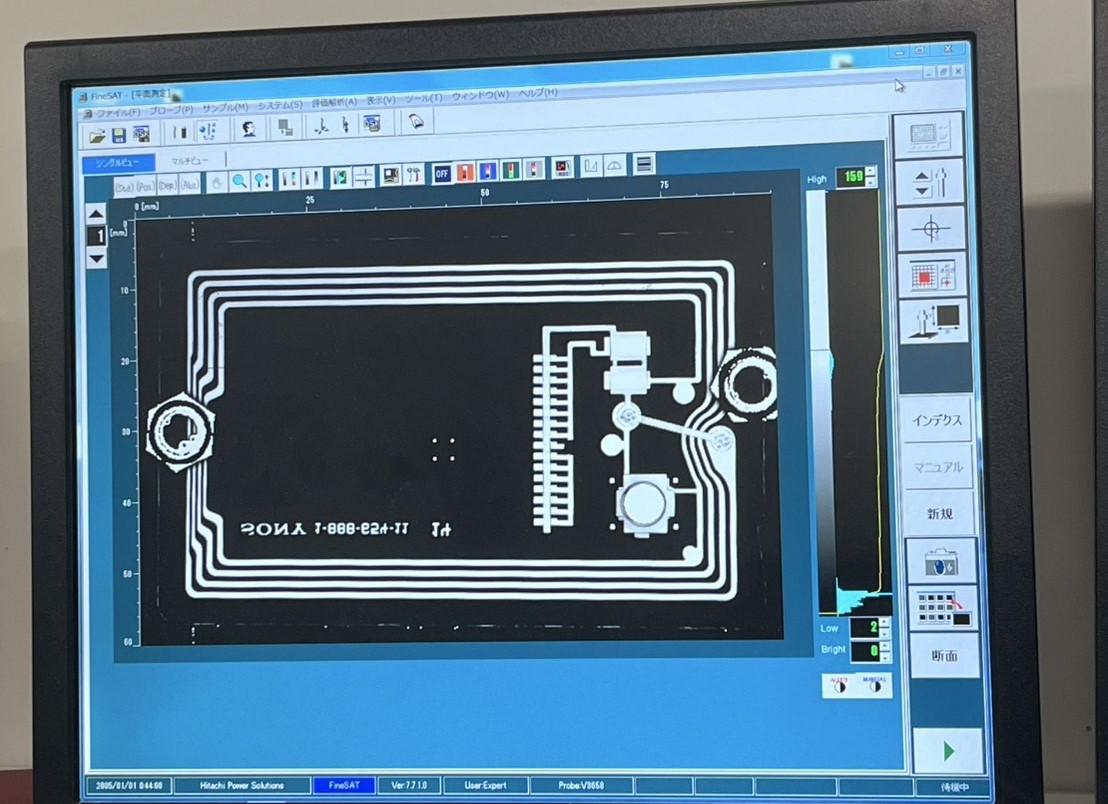
\includegraphics[width=100truemm,clip]{fig/suica.jpg}
    \caption{Circuit structure of IC card.}
    \label{fig:suica}
\end{figure}

\begin{figure}[htbp]
    \centering %中央揃え
    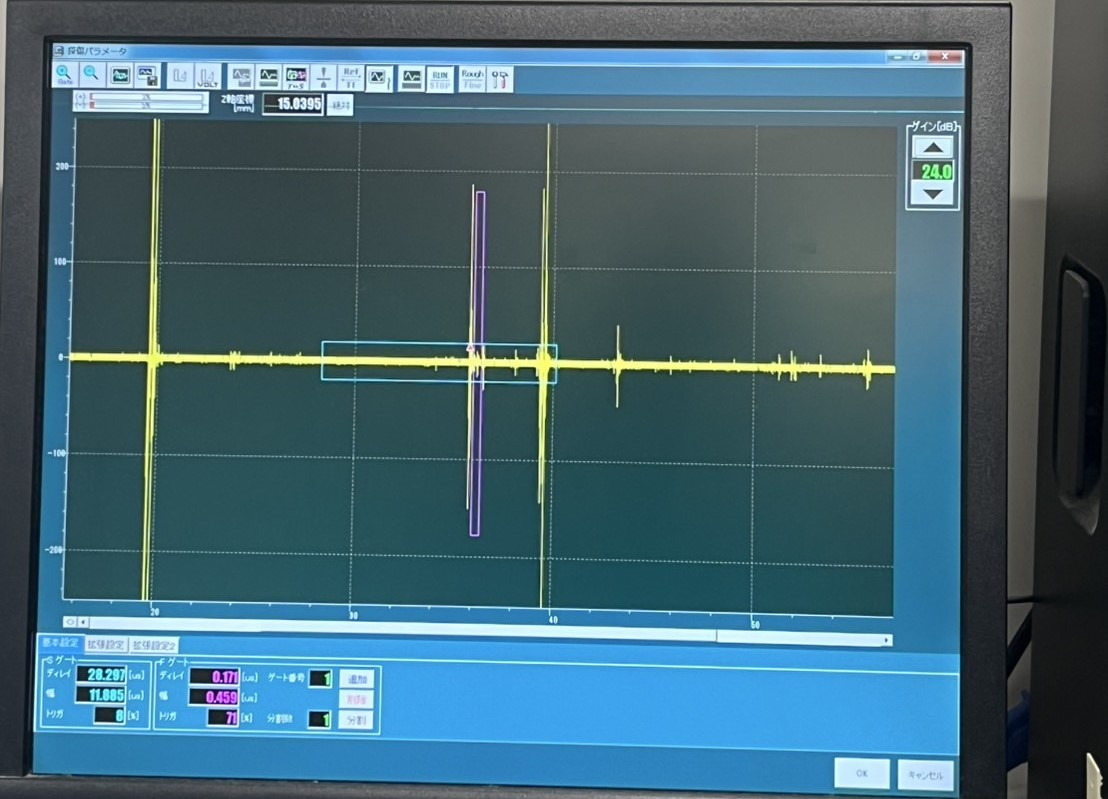
\includegraphics[width=100truemm,clip]{fig/suica波形.jpg}
    \caption{Waveform at measurement.}
    \label{fig:suica波形}
\end{figure}